\documentclass{article} % For LaTeX2e
\usepackage{nips13submit_e,times}
\usepackage{hyperref}
\usepackage{graphicx}
\usepackage{caption}
\usepackage{subcaption}
\usepackage{url}
\usepackage{multirow} 
\usepackage{cite} 

\newcommand{\specialcell}[2][c]{%
  \begin{tabular}[#1]{@{}c@{}}#2\end{tabular}}

\title{Identification of Songbird Species in Field Recordings}


\author{
Hsiao-Yu Tung \\
%Carnegie Mellon University\\
%\texttt{htung@andrew} \\
\texttt{htung@andrew.cmu.edu} \\
htung \\
\And
De-An Huang \\
%Carnegie Mellon University\\
%\texttt{deanh@andrew} \\
\texttt{deanh@andrew.cmu.edu} \\
deanh \\
\And
Xiao-Feng Xie \\
%Carnegie Mellon University\\
%\texttt{xfxie@cs} \\
\texttt{xfxie@cs.cmu.edu} \\
xfxie \\
\And
Yurui Zhou\\
%\texttt{yuruiz@andrew}\\
\texttt{yuruiz@andrew.cmu.edu}\\
yuruiz \\
\And
Joseph Russino\\
%\texttt{yuruiz@andrew}\\
\texttt{jrussino@rec.ri.cmu.edu}\\
jrussino \\
}

\newcommand{\fix}{\marginpar{FIX}}
\newcommand{\new}{\marginpar{NEW}}

\nipsfinalcopy % Uncomment for camera-ready version

\begin{document}


\maketitle

%\begin{abstract}
% The abstract paragraph should be indented 1/2~inch (3~picas) on both left and
% right-hand margins. Use 10~point type, with a vertical spacing of 11~points.
% The word \textbf{Abstract} must be centered, bold, and in point size 12. Two
% line spaces precede the abstract. The abstract must be limited to one
% paragraph.
%\end{abstract}

\section{Introduction}
%It is important to gain a better understanding of bird behavior
% and population trends. Birds respond quickly to environmental change, and may also tell us about other organisms (e.g.,
% insects they feed on), while being easier to detect. Traditional
% methods for collecting data about birds involves costly hu-
% man effort. A promising alternative is acoustic monitoring.
% There are many advantages to recording audio of birds com-
% pared to human surveys, including increased temporal and
% spatial resolution and extent, applicability in remote sites, re-
% duced observer bias, and potentially lower cost. However, it is
% an open problem for signal processing and machine learning
% to reliably identify bird sounds in real-world audio data col-
% lected in an acoustic monitoring scenario. Some of the major
% challenges include multiple simultaneously vocalizing birds,
% other sources of non-bird sound (e.g., buzzing insects), and
% background noise like wind, rain, and motor vehicles.

It is important to gain a better understanding about the climate and ecological changes in the world. One way to address this is to study seasonal migration patterns in songbird populations, since birds respond quickly to environmental changes \cite{walther2002ecological}.
During migratory periods, many species of songbirds use flight calls, which are species-specific and are distinct from other vocalizations. Therefore, flight calls information can be used to determine the relative abundance of species and is important to understand long-term population trends. Due to costly human effort to collect data about birds in traditional methods, using machine learing (ML) methods to identify bird species from continuous audio recordings has been a hot topic in in recent conference competitions.\footnote{\scriptsize ICML 2013: \href{http://www.kaggle.com/c/the-icml-2013-bird-challenge}{The Bird Challenge}; NIPS 2013: \href{http://www.kaggle.com/c/multi-label-bird-species-classification-nips2013}{
Multi-label Bird Species Classification}; MLSP 2013: \href{http://www.kaggle.com/c/mlsp-2013-birds}{Bird Classification Challenge}}. Although there are some recent advances \cite{briggs2013instance,Lasseck13,Massaron13,stattnersong13}, it is still an open ML problem to reliably identify bird sounds in field recordings data due to simultaneously vocalizing birds and various background noise \cite{BriggsMLSP13}.

In this project, we will focus on critical aspects of this problem. We start from some state-of-the-art algorithms, e.g., \cite{mlsp2,chennovel13,briggs2013instance,Lasseck13,Massaron13,stattnersong13}, adapt components to the data we have, and finally develop a scalable, integrated software tool. The total process is divided into four steps. First, Audio data are first preprocessed into spectrograms. The spectrograms are further cleaned by applying background noise reduction and image processing techniques, and connected pixels (acoustic patterns) in the spectrograms are labeled into rectangle segments. Second, features are then extracted and selected from different sources, e.g., file statistics, segment statistics and probabilistics, and mel-frequency cepstral coefficients (MFCC). Third, the classification is then done by using multiple algorithms, e.g., naive Bayes, decision trees, $k$-nearest neighbors ($k$-NN) \cite{cover1967nearest}, support vector machines (SVM) \cite{cortes1995support}, etc. Finally, we will explore some ensemble methods \cite{breiman2001random,breiman1996bagging,freund1997decision,hoeting1999bayesian,read2011classifier} for furthering improve the overall performance by combining the predictions of models, as well as facilitating scalability in real-world usages. The software developed for this project will be used by the Carnegie Museum of Natural History, and possibly shared with other land managers, researchers, and educators to enhance the use of flight calls as a method to study the populations of migratory songbirds. 

% First, we will work on segmenting flight call vocalizations within long audio files that contain other types of sounds. Second, given labeled segments of bird flight calls, we will explore possible algorithms to extract useful features and classify the corresponding songbird species automatically.
% 
%  We then etc. Finally, the classification can then be done using multiple algorithms, e.g., decision trees, support vector machines, and multi-instance multi-label learning algorithms, as well as some ensemble methods to further improve the overall performance, based on existing libraries (e.g., \href{http://scikit-learn.org}{scikit-learn}). 

%{\bf Midterm Milestone} Develop an initial workable software version and perform basic tests based on indoor voice data, after selecting suitable algorithm components that might work scalable.

%The software is scalable so that users could train it to identify flight calls from additional species and to exclude other types of background noise.

%[Yurui] Basically preprocessing and segmentation is the very first step of the bird song classification, and the methods used in preprocessing and segmentation have a big influence on classification results.

\section{Related work}

As mentioned in the Introduction, the toal process is divided into standard steps of ML components.  

The first part is about {\em preprocessing and segmentating} audio data of songbirds. Normally audio files are first processed into grayscale image by applying the Fourier transform using a Hanning or Hamming window of samples with some overlap \cite{Lasseck13, mlsp1}. Only relevent frequency range of the scope of domain interests are kept. The narrowed spectrograms are then treated as graysale images. To reduce the background noise, a {\em median clipping} method can be applied on each frequency band and time frame
% to not only remove most background noise, but also capture the sound feature clearly and precisely \cite{Lasseck13}. An alternative is to apply iterations of a whitening filter 
\cite{mlsp1}. A spectrogram can also be processed using a series of subprocesses including Gaussing filtering, local gradient, thresholding, and morphological nosing removal \cite{fodor2013ninth}. The resulting images can be further handled using standard image processing techniques such as diluation and median filter (e.g. using \href{http://scikit-image.org/}{scikit-image}). In \cite{Lasseck13}, neighboring pixels exceeding certain spatial threshold (acoustic patterns) in the spectrograms are labeled into rectangle segments. In \cite{fodor2013ninth}, small segements are discarded and remaing holes are filled. In \cite{mlsp1}, a supervised single-instance single-label classifier is used to label the probability of each pixel as bird sound or noise, and then obtain predicted segementations by applying a thershold.

The second part is about {\em feature extraction and selection}, which can have a large impact on later classification results. In \cite{mlsp1}, segement features are divided into two different categories - ``mask descriptors'' and ``profile statistics''. Histogram of gradients (HOG) have also been used \cite{mlsp1}. In \cite{fodor2013ninth}, features are obtained by applying the template matching function of scikit-image to compute the similarity at the maximum value of the normalized cross-correlation map with templates. In \cite{Lasseck13}, features come from three different sources, i.e., file statistics, segement statistics, and segment probabilities. The template matching in \href{http://opencv.org}{OpenCV library} is applied only on absolute-intensive spectrograms. Many existing work \cite{Stowell_NIPSW13,dufour2013clusterized,chennovel13,Massaron13} considers mel-frequency cepstral Coefficients (MFCC)%, which have been proved useful for speech recognition, 
as features.  Features can also be extracted using unsupervised deep learning \cite{mencialearning2013}. Addtional methods, e.g., rescaling\cite{mlsp1}, concatenation\cite{dufour2013clusterized}, bag-of-words (BoW) model \cite{Li_CVPR05}, and principal component analysis (PCA) \cite{jolliffe2005principal}, can also be used for feature engineering. 

The third part is about {\em classification}. Typical methods include naive Bayes, neural networks, logistic regression, Gaussian mixture model, radial basis function (RBF), decision trees, $k$-NN \cite{cover1967nearest}, SVM \cite{cortes1995support}, etc. Binary classifers can be turned into multi-class ones by using ome general strategies, e.g., one-versus-all and pairwise decomposition, to classify instances into multiple classes. 
Some existing methods have been used for songbird identification. In \cite{dufour2013clusterized}, a LibSVM is used in a one-versus-all fashion, and best scores have been obtained with C-SVC SVM type and linear kernel function. In \cite{mencialearning2013}, pairwise SVM, LibSVM, decision trees, and neural networks are used, and the merged SVM and RDT often leads to better results. Mutiple-instance multi-label (MIML) classsifers, e.g., MIML-SVM, MIML-RBF, MIML-$k$NN are considered in \cite{mlsp1}. 

Finally, different {\em ensemble learing} methods have also been used for combining the predictions of several models. In theory, ensembles can be more flexibility in the functions they can represent. Typical methods including gradient boosting (GB) \cite{friedman2001greedy}, random forest (RF) \cite{breiman2001random}, extremely randomized trees (ERT) \cite{geurts2006extremely}, bootstrap aggregating (or bagging) \cite{breiman1996bagging}, bayesian model averaging (BMA) \cite{hoeting1999bayesian}, and ensemble of classifier chains (ECC) \cite{read2011classifier}. Some of them, e.g., GB \cite{chennovel13}, RF \cite{Stowell_NIPSW13,chennovel13,fodor2013ninth}, 
ERT \cite{Lasseck13}, have been directly used for songbird identification. There are also some hybrid methods. In \cite{chennovel13}, GB and RF are combined by a simple linear blending method, where the final prediction is given by a linear combination of ensemble predictions, and the combination coefficients are determined by a Lasso and elastic-net regularizion of generalized linear model. In \cite{Massaron13}, an ensemble of logistic regression and GB classfiers are considered. In \cite{mlsp2}, an ensemble of classifier chains with RF is applied.

Many classification and ensemble methods can be obtained in \href{http://scikit-learn.org}{scikit-learn library}. 

\section{Methods}

\subsection{Preprocessing}

[Yurui]
% In preprocessing we first re-sampled the audio files to 22050 Hz guarantee a uniform audio sample format for all training and test data. For each audio file we split it into 256 segments. Then the Power Spectral Density of each segments can be calculated. For each segments we use a Hanning window with \%75 overlap. Finally, the spectrogram of each audio file is treated as gray-scale image for further noise reduction and segmentation.
% 
% Notice the case that in a processed grayscale image most area was occupied by the random noise. What we want is to get rid of the background noise completely and increase the contrast between real signal and the background. Given the several different algorithm tested, the best one is the so called Median clipping algorithm. The idea is simple, for each pixel we compute the median and variance of its corresponding row and column. If the pixel is above the median plus three times variance we set the pixel value to 1, otherwise the value would be set to 0. The median clipping algorithm works best because it not only removes most background noise, but also capture the sound feature clearly and precisely.
% 
% Such a algorithm, though perform well in noise removing and feature capturing, requires large amount of computation because the average and variance of each column of the row need to be calculated. Given the huge size of the processed grayscale image, we need a more efficient algorithm to segment the image. Thus further experiments is needed to explore an balance point between noise reduction effectivity and efficiency.
% 
% Similar to the methods used in \cite{Lasseck13}, we apply standard image processing techniques to further reduce residual noise dots. Finally we would use find connected pixels from the image and label the segments.

\subsection{Features}
\label{sec:Features}

Features can have a large impact on classification results. For this project, we have chosen to implement a large set of features used in previous successful attempts at birdsong classification. We will ultimately choose a smaller subset of these features that provide the most discriminatory power. 


\textbf{Mel-Frequency Cepstral Coefficients}
While flight calls recognition is a new application, audio recognition is a well developed area in signal processing. We will build features based on MFCCs, which are commonly used as features in speech recognition systems, but can be sensitive to the presence of noise \cite{tyagi2005desensitizing}; for this reason, we expect that they may be
useful features for classifying the clear lab data but less useful for the noisy outdoor data. A temporal signal is first transformed into a series of frames where each frame consists of a 13-dimensional MFCC vector, using Wojcicki's MATLAB
implementation. \footnote{\scriptsize \href{http://www.mathworks.com/matlabcentral/fileexchange/32849-htk-mfcc-matlab/content/mfcc/mfcc.m}{HTK MFCC MATLAB} by K. Wojcicki: Mel frequency cepstral coefficient feature extraction that closely matches that of HTK's HCopy.}. Each frame represents a duration of 12ms. The step size is 4ms. We also include the fist and second derivatives of MFCCs, which results in a 39 (13$\times$3) dimensional vector for each frame.

\textbf{Bag-of-Words Model over MFCCs}
\label{sec:bow}
In contrast to \cite{Dufour_NIPSW13}, which assumes that the number of frames is fixed for all audio segments to classify, we make no assumption on the length of the audio segment, since the length of flight calls might variate. In this case, we want a feature that is temporally scale invariant. Intuitively, even when a flight call is temporally scaled (extended or shorten), it should still be classified as the flight call of the same species. We leverage the progress in image classification and applied the bag-of-words (BoW) model \cite{Li_CVPR05} over our MFCCs. By treating audio features (MFCCs in our case) as `words', each audio segment is represented by a sparse vector of occurrence counts of words in BoW model; that is, a sparse histogram over the vocabulary.

We learn the vocabulary, also called the codebook, by performing k-means clustering over sampled training MFCCs. Codewords are then defined as the centers of the learned clusters. In test time, we extract MFCCs from the test audio segment and quantize the 39 dimensional MFCCs to a learned codeword. The audio segment is represented by a $K$ dimensional histogram over the codeword, where $K$ is the size of the codebook. 

One limitation of BoW model on audio segment is that the temporal information are lost in the model. However, as shown in the experiments, BoW is able to achieve satisfactory classification result on single-label single-instance case. We are considering to build higher order N-gram model on the learned vocabulary to capture the temporal information.

% \textbf{Other features}
% The other features that we intend to explore can be classified broadly into two categories: spectrum-wide features and
% segment features. The spectrum-wide features describe qualities of the full spectrograph for a given recording, while
% the segment features describe qualities of individual segmented portions of the spectrograph. In addition, we plan on using the min, max, average, and standard deviation of frequency values over
% the entire spectrograph, and on dividing the spectrograph into $N$ equally spaced frequency bands and taking the same
% statistics for each frequency band as features. Lasseck had success with this method in 2013 using $N=16$ \cite{Lasseck13}.
%   For segment features, we will use the same basic statistics on a per-segment basis. In addition, we will explore the
% usefulness of many of the other segment features that were used successfully in \cite{mlsp1}. These can be divided 
% into two different categories - ``mask descriptors'', which describe the general shape of a segment, and ``profile statistics'', 
% which describe the frequency and time profiles within segments. The mask descriptors include bandwidth,duration, area, 
% perimeter, non-compactness, and rectangularity; the profile statistics include profile uniformity, mean, variance,
% skewness, and kurtosis. The final set of segment features that we will explore are the Histogram of Gradients (HOG), 
% which have successfully been used for songbird classification \cite{mlsp1,fodor2013ninth}. 

\subsection{Classifiers}
We consider several classifiers/regressors.

\textbf{Nearest Neighbor (NN).} For each testing data, the NN classifier finds the nearest training data point and transfer the corresponding label. The NN classifier directly reflect the effect of our features and is used as baseline. Depends on the features, different distance metric should be used. We will compare the performance of euclidean and $\chi^2$ distance on the BoW feature in the experiments.

\textbf{Support Vector Machine (SVM).} The most common approach for multi-label classification is to use an ensemble of binary classifiers, where each classifier predicts if an instance belongs to
one specific class or not. SVMs trained in a pairwise fashion has obtained state-of-the-art results on standard multi-label benchmark datasets \cite{Mencia_NIPSW13}. Furthermore, we will be able to integrate different kernels to improve the performance using the SVM. For example, the $\chi^2$ kernel will have a better performance for histogram than the linear kernel. We also consider support vector regression to produce soft output for ensemble learning.

%textbf{Support Vector Regression (SVR).} We use SVR to produce a soft output version of SVM

\textbf{Random Forest.} Random forests has been widely used for multi-label classification \cite{Lasseck13, chennovel13, Stowell_NIPSW13, Zhang_SDM2010}.
Random Forest is operated by constructing decision tree structure by the training examples. One of the popular algorithm is tree bagging, in which the training process includes repeatedly selecting a bootstrap sample of the training set and  fitting the trees to them. After the training process, the label decision is made either on the majority of the votes or a weighted combination from individual trees.

%\textbf{Naive Bayes.} 

\textbf{Logistic Regression.} Ensemble of logistic regression has been used for multi-label bird song classification \cite{Massaron13} because of its simplicity. We also consider this method as the baseline for soft output.

\subsection{Ensemble Learning}


\section{Experiments}

We first evaluate our system on single-label data to see if the flight calls are separable using our method.

{\bf Data Set} Large amounts of audio data (about 20 terabytes) for bird calls have been collected. The data contain flight calls from approximately 20-30 species of songbirds, examples of other background noises, and long audio files that contain flight calls (some of them might be too faint to identify them to species) and other background sounds. The software developed can be tested using long audio files where all the flight calls of songbirds have been detected, and with manual identification by Amy Tegeler, an Avian Ecologist from the Carnegie Museum of Natural History.

\textbf{Data.}  We use the flight calls of songbirds manually segmented and labeled by Amy Tegeler, an Avian Ecologist from the Carnegie Museum of Natural History, to evaluate the performance of our system on indoor flight calls classification. We used the data from year 2008 to 2013. The total number of species is 32. But only 11 species has more than 100 data. Therefore, the experiment is performed on those 11 species, and 100 data points are randomly sampled from each species. The 100 data points are randomly partitioned into 20 testing data and 80 training data for each species.

\textbf{Segmentation.}
Since the flight call segments are already manually identified, we do not perform segmentation in this experiment.

\textbf{Features.}
We use the BoW over MFCCs in Section \ref{sec:Features} as the features for this experiment. The size of the code book is 200, and the MFCCs consider the frequencies from 1500 Hz to 22000Hz.

\textbf{Classifiers.}
Before beginning with the training process, we first examine the property of the data. We can see that most of the value in the original data is zero. After taking the log value of the data, we can find that a small group of the data is separated from the others. In some of the dimension, this small contains only a number of specific species of birds, which might be helpful in the classification.
\begin{figure}[ht!]
    \centering
    {(a)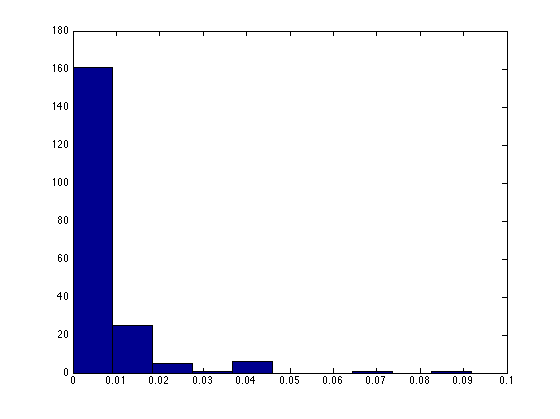
\includegraphics[width=0.45\linewidth]{../Figure/Train_features}
    (b)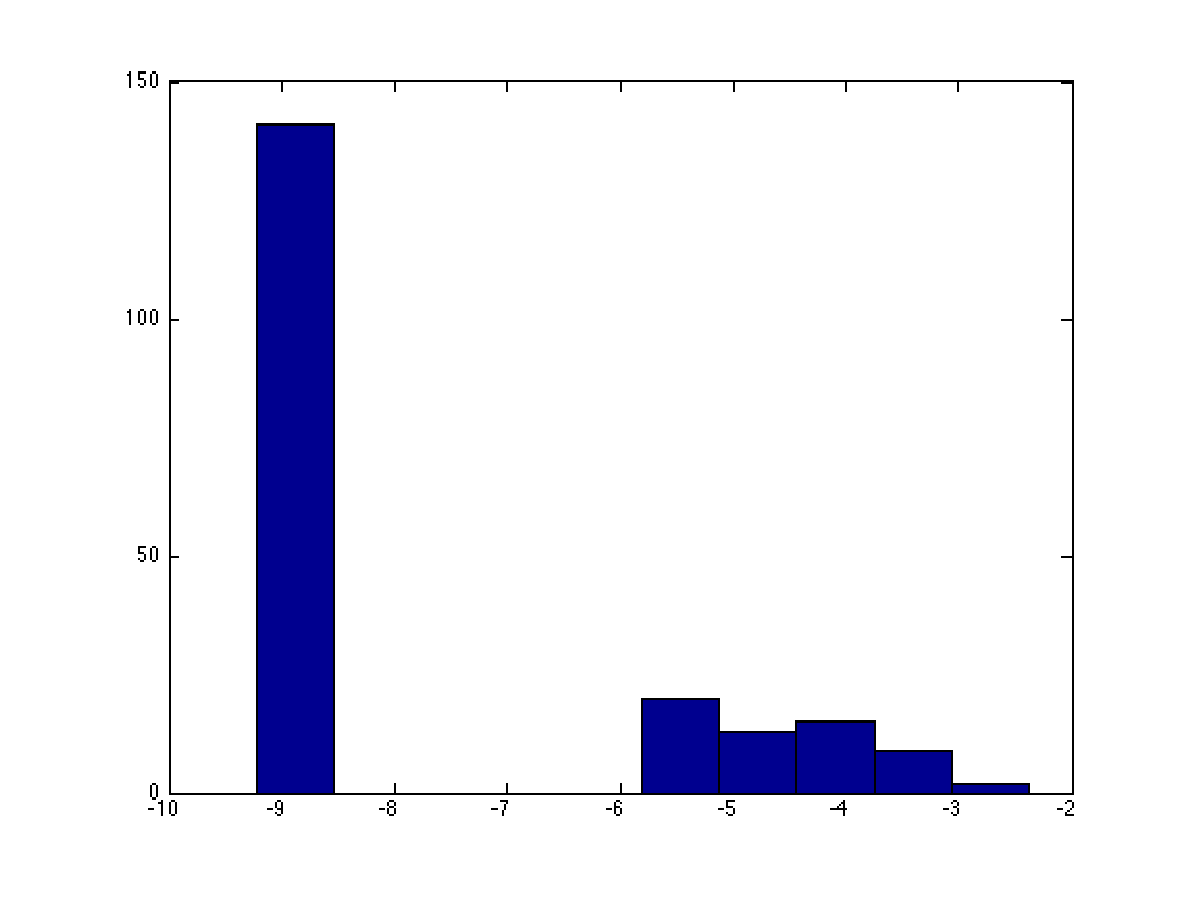
\includegraphics[width=0.45\linewidth]{../Figure/Train_features_log}}
    \caption{(a) is the histogram of second feature. Most of the values are close to zero. (b) is the histogram of the log value of the original data.}
    \label{fig:hist}
\end{figure}


We compare the results using nearest neighbor, support vector machine, random forest and naive bayes classifier.


\begin{table}[t]
\caption{Accuracy of different classifier}
\begin{center}
\begin{tabular}{|c|c|c|c|c|c|}
\hline
   classifier  & setting      &accuracy   & classifier    & setting      & accuracy\\
\hline
KNN     & chi-square    &62.27      &     &chi-square kernel  &72.73\\ \cline{2-3} \cline{5-6}
(distance) & euclidean     &54.09      &   SVM    & RBF               &70\\ \cline{1-3} \cline{5-6}
       &               &     &    (kernel types)    & linear            &67.7273\\ \cline{1-3} \cline{5-6}
Naive Bayes  & kernel density  & 15.91           &       & polynomial        &69.0909\\ \cline{1-3} \cline{5-6}
 RandomForest &         & 7.27                 &       & Sigmoid           &70.9091\\ \hline
\end{tabular}
\end{center}
\end{table}

We can see from our results that kernel SVM has better performance than the other method. First we show the parameter selection in using RBF kernel. Figure \ref{fig:RBF} shows the accuracy to the penalty term $C$ and the parameter $\gamma$. The parameter we selected are $\gamma = 15$ and $C = 4000$.

\begin{figure}[ht!]
    \centering
    {(a)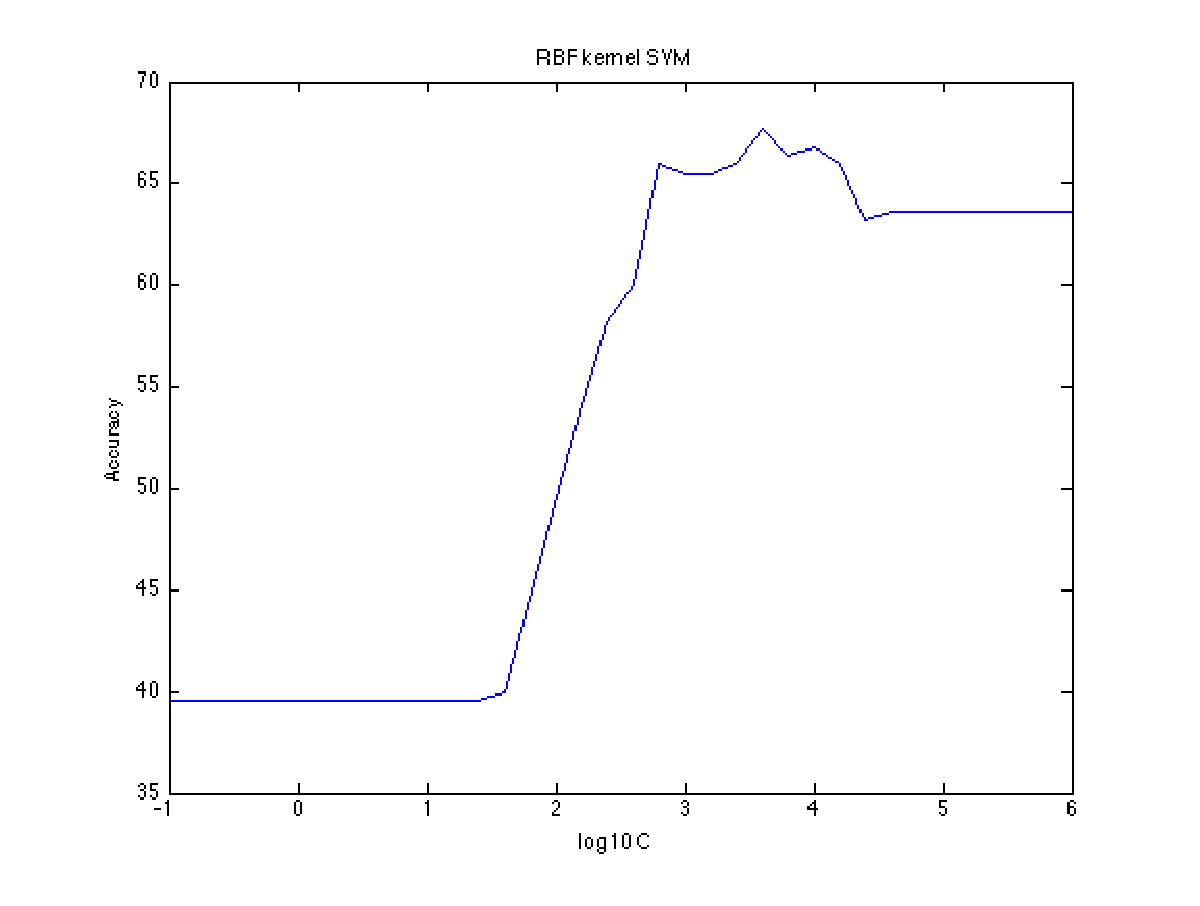
\includegraphics[width=0.45\linewidth]{../Figure/RBF_cost_accuracy}
    (b)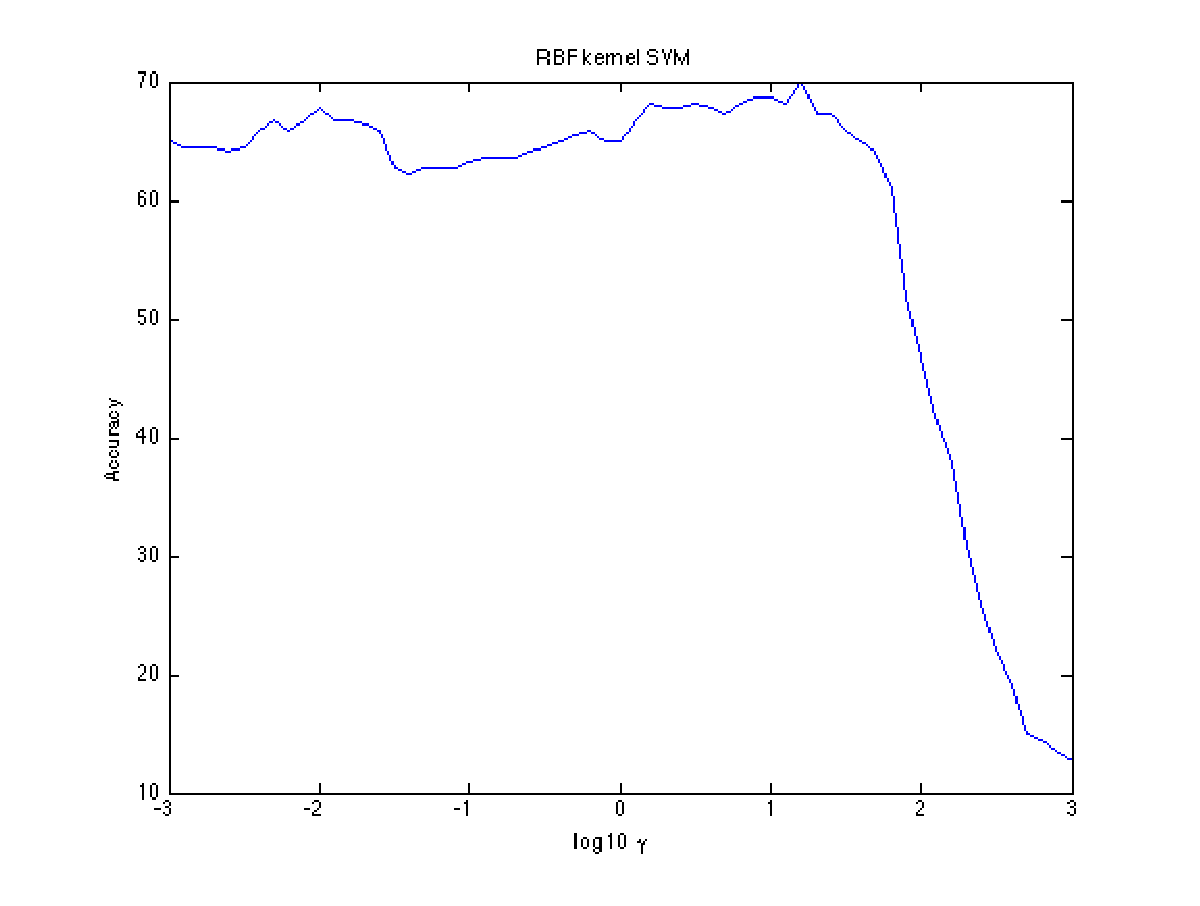
\includegraphics[width=0.45\linewidth]{../Figure/RBF_gamma_accuracy}}
    \caption{(a) Accuracy to penalty term c. (b) Accuracy to parameter $\gamma$. }
    \label{fig:RBF}
\end{figure}

In considering that original feature distribution is not a Gaussian distribution, for $x_i,j$ representing the $j^{th}$ feature in the object $i$, we first use a log transformation such that $x_{i,j} = log(x_{i,j} + 0.0001)$ to make the feature distribution more like a combination of Gaussian distribution (see \ref{fig:hist}(b)). The operation leads to a 1.27 improvement in the accuracy after parameter selection process.


\begin{figure}[ht!]
    \centering
    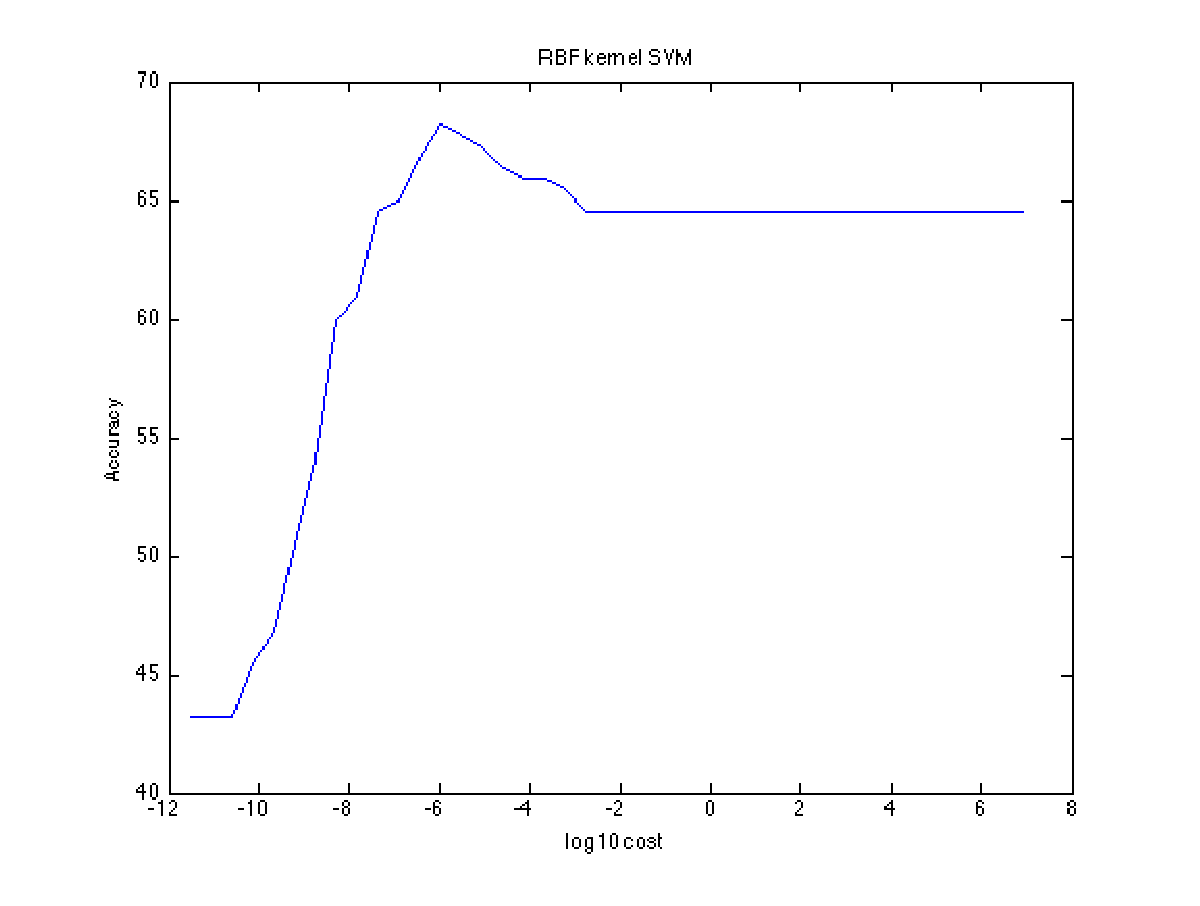
\includegraphics[width=0.45\linewidth]{../Figure/RBF_cost_accuracy_log}
     \centering
    \caption{Accuracy to penalty C after log transformation on the original feature.}
\end{figure}

Next, we show the results for applying SVM with polynomial kernel. Figure \ref{fig:poly} shows that the performance of accuracy to penalty C is similar to RBF kernel and the optimal value of this parameter is 16000. Besides, according to the experiment results, the optimal degree for the data is around 2. The reason might due to small data size that we use recently so that increasing model complexity will lead to overfitting problem. So we focus on simple model for recent data.  
 
\begin{figure}[ht!]
    \centering
    {(a)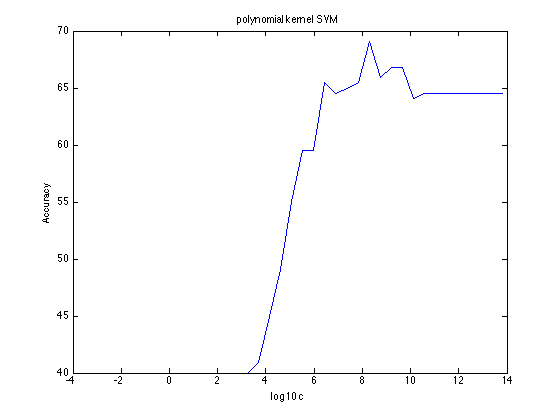
\includegraphics[width=0.45\linewidth]{../Figure/Poly_cost_accuracy}
    (b)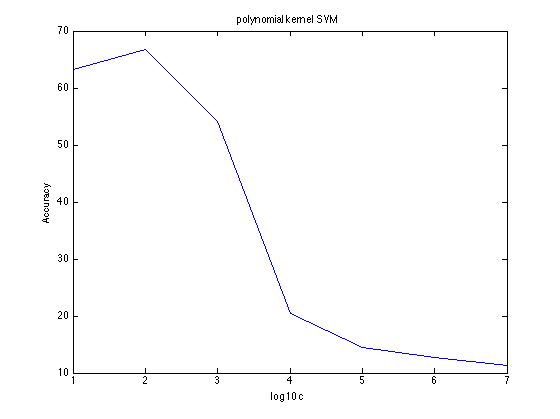
\includegraphics[width=0.45\linewidth]{../Figure/Poly_degree_accuracy}}
    \caption{(a) Accuracy to penalty term c. (b) Accuracy to parameter degree d}
    \label{fig:poly}
\end{figure}

The reason why random forest and naive Bayes failed is that the training example for each species is now limited to 80. From the predicted classification labels from the results of random forest, we found that the identities in some of the class are all mis-classified into another class, which means that the tree is ill-trained and biased such that many cases will be made to the same decision. 

\bibliographystyle{abbrv}
\bibliography{../bib/birds,../bib/ml}

\end{document}
